\chapter{Evaluation}

\section{Event Detection Evaluation}
\subsection{Evaluation Data and Metric}
The evaluation for event detection uses data from IEEE AASP Challenge for event detection\footnote{http://c4dm.eecs.qmul.ac.uk/sceneseventschallenge}.  
In this challenge, a training dataset are given containing instantiations of individual events for 16 different classes. 
Moreover, there is also a developement dataset, which consist of 1 minute recordings of every-day audio events in a number of office environments. 
This developement dataset is annotated by human and can be used for model evaluation. \\ 

The evaluation begins by first segmenting clips using the a segmenter. 
We assume that only one event happens during a segment. 
Then use the trained GMM to calculate the posterior probability. 
The detected event is chosen when its corresponding GMM has the highest posterior probability.\\ 
 
Three types of assessment of the various systems will take place, i.e., a frame-based, event-based, and class-wise event-based evaluation \cite{giannoulis2013database}.  These three metrics differ mainly in the way they interpret a sequence result of detected events.  
Suppose $r$, $e$ and $c$ denotes number of ground truth, estimated and correct events, the Precision, Recall, and F-measure are defined as: 
\begin{equation}
	P = \frac{c}{e}, R = \frac{c}{r}, F = \frac{2PR}{P+R}.  
\end{equation}
For the frame-based metric, $r$, $e$, and $c$ are calculated in a 10ms window and are averaged over the entire duration. 
The event-based metric takes a different perspective of how a event unit is calculated. 
Unlike frame-based metric, which undiscriminately count event for every 10ms, this metric focuses on the true onset and offset time of ground truth events. 
Onset-only evaluation set restriction on onset time tolerance. 
Onset-offset evaluation further add a offset time restriction. 
The onset-only and onset-offset evaluation are averaged as event-based metric. 
Class-wise event-based calculate $r$, $e$, and $c$ for each class separately. And then it is averaged over classes. 
Finally, the F-measure for these three metric are averaged as the final metric of a system, and we will compare this metric with other systems. 

\subsection{Evaluation Process}
The evaluation takes on two parts: self tuning and system comparison. \\ 

Audio events are detected using the previous proposed GMM method, but there are still some parameters or configuration to be tuned for the best performance of our model.
Most importantly, the number of component number in GMM are ser by human, we run a evaluation for different component numbers from 4 to 45 to see how the number affects the F-measure. \\ 

In system comparison, we use other models from the aforementioned IEEE AASP Challenge\footnote{http://c4dm.eecs.qmul.ac.uk/sceneseventschallenge/resultsOL.html}. 
In the submitted papers, contestents also carried out the same evaluation on the developement dataset, so the comparison are done on the same dataset.  

\subsection{Evaluation Result}
The following picture is the result of average F-measure with regard to different component numbers in GMM. 
% component.eps
\begin{figure}[htb]
\centering
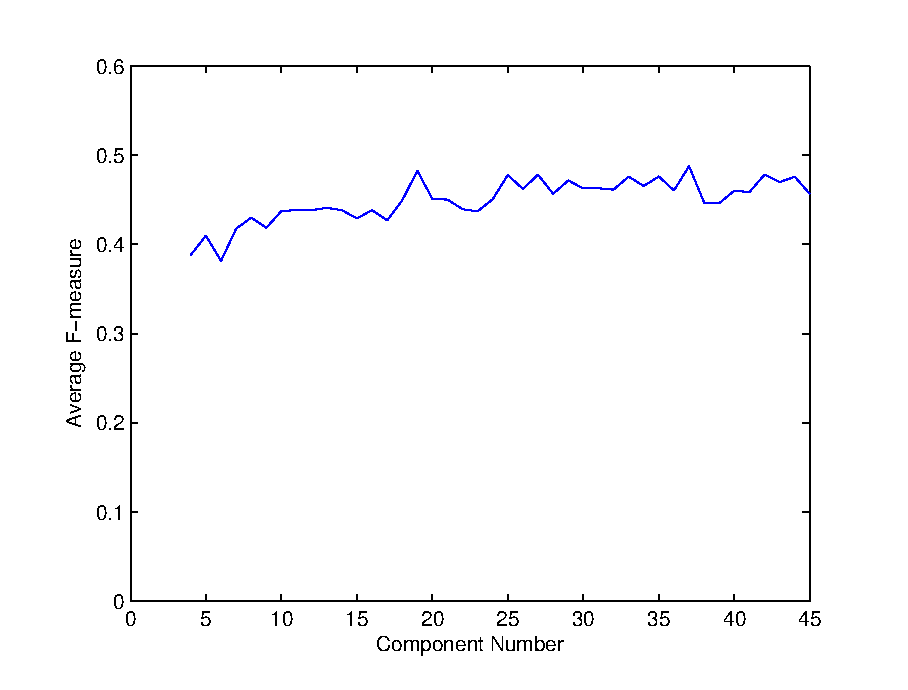
\includegraphics[scale=0.85]{figure/evaluation/component}
\label{fig:component}
\end{figure}

As we can see in this picture, the F-measure gradually rise when component number are increasing. 
But after component number reaching 18 or so, the F-measure roughly stays the same. \\ 

% running time eps 
\begin{table}[htb]
\centering
\caption{Event Detetion Evaluation}
\begin{tabular}{lllll}
\hline
         & EB    & CWEB  & FB    & Average \\
\hline
baseline & 15.4  & 13.5  & 20.6  & 16.50   \\
NR2      & 11.06 & 20.9  & 32.49 & 21.48   \\
NVM      & 47.53 & 41.28 & 54.41 & 47.74   \\
Our      & 53.44 & 40.07 & 52.41 & 48.64   \\
VVK      & 51.13 & 39.77 & 56.28 & 49.06   \\
GVV      & 46.8  & 36.7  & 65.2  & 49.57   \\
DHV      & 51.05 & 38.05 & 61.6  & 50.23   \\     
\hline
\end{tabular}
\end{table}

Moreover, figure X-X is the running time of our system with regard to the number of components. 
There is basically a linear relationship between the number of components and the total running time. 
Hence, we choose to use 18 as the component number for our system, since this component number has a good F-measure, and the speed for training models are also fast.\\ 



\section{Scene Recognition Evaluation}

\section{Summary}
